\section{Standard Bangla license plate}
\subsection{Vehicle types}
There are many different types in Bangladesh, e.g.: private car, auto-rickshaw, pick up/van, delivery van/truck, ambulance/mobile dispensary, microbus, articulated truck, micro-bus etc. Vehicles considered in this thesis are listed in Table \ref{tab:vechicleClasses}. There were no previous format and standardization of the license plate. But recently the government has enforced digital license plate for all vehicles.

  
\begin{table}[htb]
	\centering
	\begin{tabular}{|c|c|c|c|c|}
		\hline
		Serial & Identifier & Begin Number & End Number & Type \\
		\hline
		1  & MA  & 51 & 99 & Delivery van/truck \\ 
		\hline
		2  & THA & 11 & 99 & Pick up/van \\ 
		\hline
		3  & CAA & 11 & 99 & Ambulance/Mobile dispensary \\ 
		\hline
		4  & U	 & 11 & 99 &	Cargo truck \\ 
		\hline
		5  & TA	 & 11 & 99 & Heavy truck \\ 
		\hline
		6  & GA  & 11 & 99 & Motor Car \\ 
		\hline
		7  & RA	 & 11 & 99 & President's office car \\ 
		\hline
		8  & ZA	 & 11 & 99 & Pm’s office (Any vehicle) \\ 
		\hline
		9  & DHA & 61 & 80 & Articulated truck \\
		\hline
		10 & CHA & 11 & 50 & Micro-bus \\ 
		\hline
		11 & PA	 & 11 & 99 & Taxi Cab \\ 
		\hline		
	\end{tabular}
	\caption{Vehicles class in our consideration (provided by BRTA \cite{brta}).}
	\label{tab:vechicleClasses}
\end{table}

License plates also have different colors based on vehicle class as shown in Table \ref{tab:colorsByCategory}.
\begin{table}[hb]
	\centering
	\begin{tabular}{|m{3cm}|m{3cm}|m{3cm}|m{4cm}|}
		\hline
		Vehicle Category & Plate Color & Character Color & Sample \\ 
		\hline		    
		Private & Black & White 
		& 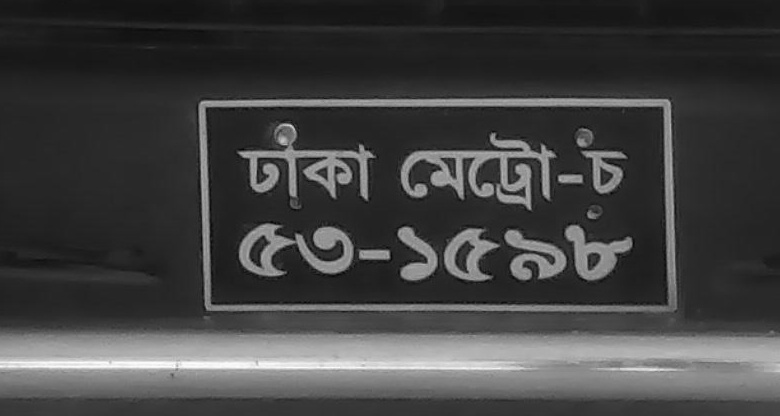
\includegraphics[width=4cm]{./img/experiment/stage.9/00-private2}
		\\ \hline
		Commercial  & White & Black &
		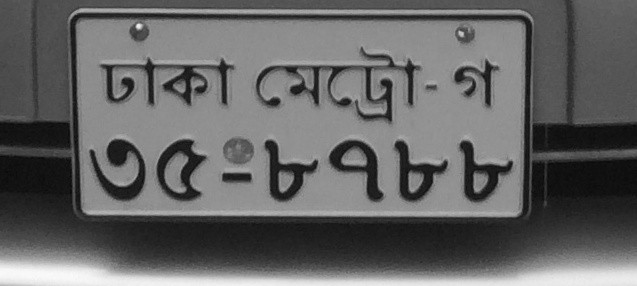
\includegraphics[width=4cm]{./img/experiment/stage.9/00-good}
		\\ \hline		
	\end{tabular}
	\caption{Different colors of plate for different vehicle category}
	\label{tab:colorsByCategory}
\end{table}





\subsection{Structure of the plate}
The digital Bengali license plate is normally written in two lines (see Figure \ref{fig:EX}).

\begin{figure}
\centering
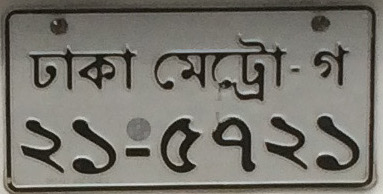
\includegraphics[scale=0.8]{./img/sample_plate}
\caption{Example of a digital license plate in Bangla}
\label{fig:EX}
\end{figure}

As the example given the line on the top written in Bangla and the bottom line has all digits in Bangla.    

\subsection{Parts of plate number}[h]
Figure \ref{fig:UP} got two parts. First part before the '-' denotes the city of the car license and then the second part denotes the series it is in.

The bottom part in Figure \ref{fig:DOWN} is the number of the license assigned to the particular vehicle by the licensing rules and regulation of Bangladesh Road Transport Authority.

\begin{figure}
\centering

\includegraphics[scale=0.6]{./img/up}
\caption{Upper portion of a license plate}
\label{fig:UP}


\includegraphics[scale=0.6]{./img/down}
\caption{Bottom portion of a license plate}
\label{fig:DOWN}
\end{figure} 

    
\subsection{Plate fonts}
Digital license plate is offering verified fonts, but in Bangladesh those rules are not strictly followed by all vehicle owners. Also the current dataset does not have any universal font. So, the fonts can be different but easily understandable for this thesis work.

\begin{figure}
\centering
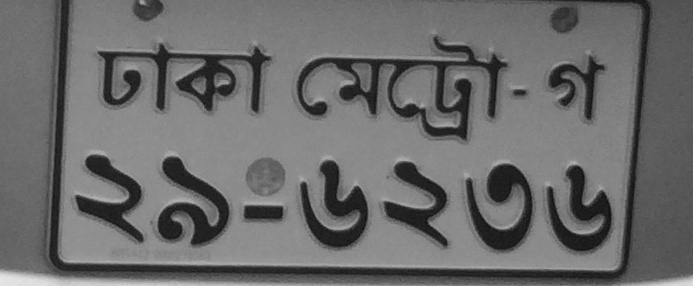
\includegraphics[width=0.5\linewidth]{./img/experiment/stage.9/00-angle2}
\caption{A standard license plate with standard font}

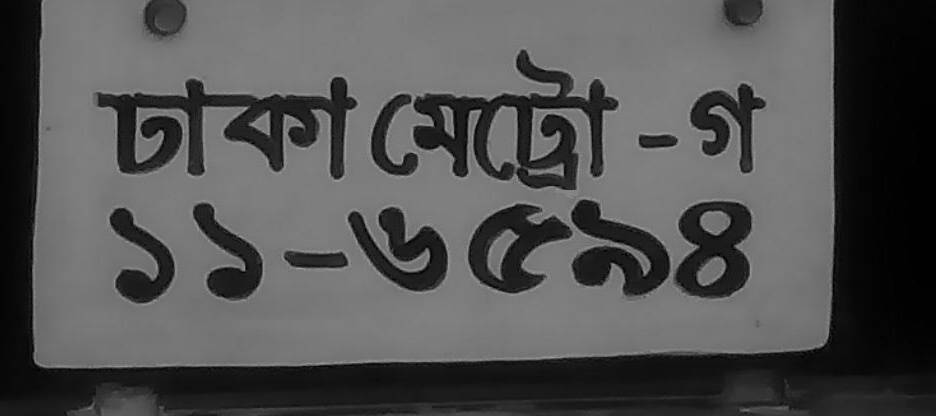
\includegraphics[width=0.5\linewidth]{./img/experiment/stage.9/00-badfont}
\caption{A standard license plate with non-standard font}
\end{figure} 
